\documentclass[10pt, a4paper]{article}
\usepackage{graphicx}
\usepackage{geometry}
 \geometry{
 a4paper,
 total={170mm,257mm},
 left=20mm,
 top=20mm,
 }
 
\title{Is Florida getting warmer}

\author{Junyue Zhang}

\date{10-25-2021}

\begin{document}
  \maketitle
  
  \section{Results}
    The correlation coefficient between years and temperatures is calculated as 0.533. And this calculation is repeated 10000 times, each time the temperatures are randomly reshuffled and the correlation coefficient is recalculated. The random correlation coefficients are continuously appended in a new vector. Then the fraction of the random correlation coefficient greater than 0.533 is considered as the approximate, asymptotic p-value. 
    Thus, the p-value is calculated as zero.  
   
  \section{Discussion}
    The p-value indicates the probability that the occurrence of an observed difference just by random chance. The lower p-value is related to the greater statistical significance of the observed difference.
    In this case, the p-value is less than 0.01, which means the difference between Florida temperature and years is significant.
    It can be speculated that the temperatures of Florida are increasing with years.  
    Therefore, Florida is considered getting warmer over years.

  \section{Conclusion}
    After applying a distribution of random correlation coefficients between Florida temperature and time, it can be concluded that Florida is getting warmer over years.

\begin{figure}[h]
  \centering
  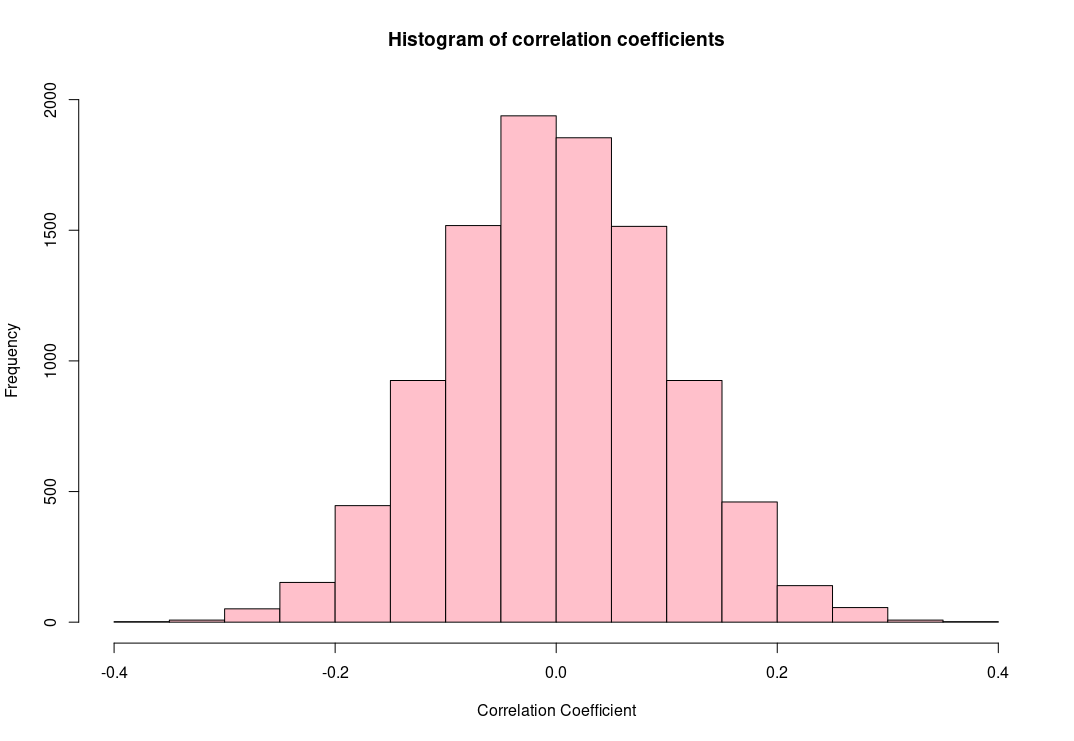
\includegraphics[scale = 0.3]{../data/histogram_of_rcc.png}
  \caption{Histogram of Correlation Coefficients}
  \label{figure1}
\end{figure}
Figure \ref{figure1} shows a histogram of correlation coefficients.


\end{document}